% Báo cáo tiến độ 06/10/2026 — build: latexmk (XeLaTeX, xem latexmkrc)
\documentclass[aspectratio=169,11pt]{beamer}

\usepackage{fontspec}
\setsansfont{Lato}
\newfontfamily\sym{DejaVu Sans}
\usepackage{booktabs}
\usepackage{array}
\usepackage{tikz}
\usetikzlibrary{arrows.meta,calc,positioning}
\usepackage{pgfplots}
\pgfplotsset{compat=1.18}

% ---------- màu ----------
\definecolor{ink}{HTML}{1F2328}
\definecolor{mute}{HTML}{8A9099}
\definecolor{line}{HTML}{D5DAE1}
\definecolor{accent}{HTML}{2F6FB3}
\definecolor{hot}{HTML}{E07B24}
\definecolor{ok}{HTML}{2E9E5B}

% ---------- giao diện tối giản ----------
\setbeamertemplate{navigation symbols}{}
\setbeamercolor{normal text}{fg=ink,bg=white}
\setbeamercolor{structure}{fg=accent}
\setbeamercolor{frametitle}{fg=ink}
\setbeamercolor{title}{fg=ink}
\setbeamerfont{frametitle}{size=\Large,series=\bfseries}
\setbeamerfont{title}{size=\LARGE,series=\bfseries}
\setbeamertemplate{frametitle}{%
  \vspace*{0.7em}\insertframetitle\par\vspace{0.25em}%
  {\color{accent}\rule{1.2cm}{2pt}}\par}
\setbeamertemplate{footline}{%
  \hfill{\scriptsize\color{mute}\insertframenumber}\hspace*{1.2em}\vspace*{0.8em}}
\setbeamertemplate{itemize item}{\color{accent}\small$\bullet$}
\setbeamertemplate{itemize subitem}{\color{mute}\scriptsize$\bullet$}
\setlength{\parskip}{0pt}

\setbeamertemplate{title page}{%
  \vspace*{1.4cm}
  {\color{accent}\rule{1.5cm}{3pt}}\par\vspace{0.5cm}
  {\usebeamerfont{title}\usebeamercolor[fg]{title}\inserttitle\par}
  \vspace{0.35cm}
  {\large\color{mute}\insertsubtitle\par}
  \vfill
  {\insertauthor\par}\vspace{0.1cm}
  {\small\color{mute}\insertinstitute\quad·\quad\insertdate\par}
  \vspace*{0.9cm}}

\newcommand{\done}{{\sym\color{ok}✓}}
\newcommand{\half}{{\sym\color{hot}◐}}
\newcommand{\todo}{{\sym\color{mute}○}}
\newcommand{\gray}[1]{{\color{mute}#1}}

\title{Học chính sách hành động cộng tác\\người -- robot có nhận thức ý định}
\subtitle{Báo cáo tiến độ}
\author{Đào Duy Hưng}
\institute{GVHD: PGS.TS. Hoàng Văn Xiêm}
\date{06/10/2026}

\begin{document}

% =====================================================================
\begin{frame}[plain]
  \titlepage
\end{frame}

% =====================================================================
\begin{frame}{Bối cảnh}
  \begin{columns}[c]
    \column{0.52\textwidth}
      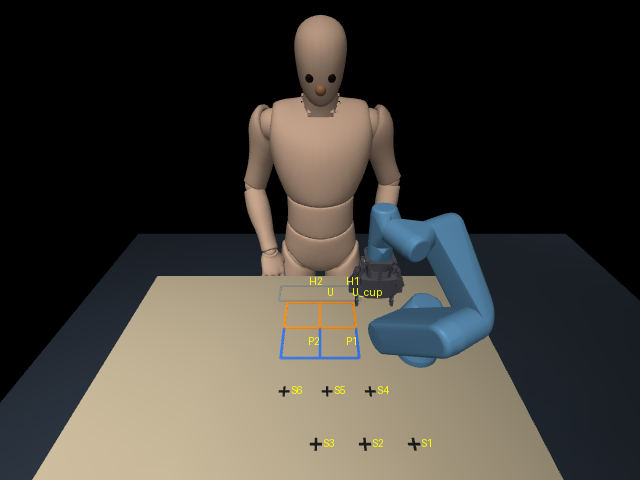
\includegraphics[width=\linewidth]{figures/scene.png}
    \column{0.44\textwidth}
      {\Large Robot làm việc \textbf{cùng người}}\par
      \vspace{1.2em}
      Robot cần biết:\par\vspace{0.6em}
      \begin{itemize}\setlength{\itemsep}{0.6em}
        \item \textbf{Làm gì?} \gray{\small ngữ nghĩa}
        \item \textbf{Ở đâu?} \gray{\small không gian}
        \item \textbf{Khi nào?} \gray{\small thời gian}
      \end{itemize}
  \end{columns}
\end{frame}

% =====================================================================
\begin{frame}{Động lực}
  \centering
  \vspace{0.6em}
  \begin{tikzpicture}[font=\small, scale=0.95, every node/.style={transform shape}]
    % trục thời gian
    \draw[-{Stealth}, mute, thick] (0,0) -- (10,0) node[right] {\gray{thời gian}};
    \draw[dashed, line, thick] (1,0) -- (1,2.6);
    \draw[dashed, line, thick] (4.5,0) -- (4.5,2.6);
    \node[below, align=center] at (1,-0.1) {người bắt đầu\\chỉ tay};
    \node[below, align=center] at (4.5,-0.1) {ý định\\rõ ràng};
    % chờ rõ ý định
    \node[anchor=east] at (-0.2,2.0) {Chờ rõ ý định};
    \fill[mute!75, rounded corners=2pt] (4.5,1.75) rectangle (9,2.25);
    \node[white, font=\small\bfseries] at (6.75,2.0) {robot làm};
    % phản hồi sớm
    \node[anchor=east] at (-0.2,0.9) {Phản hồi sớm};
    \fill[accent, rounded corners=2pt] (1.5,0.65) rectangle (6,1.15);
    \node[white, font=\small\bfseries] at (3.75,0.9) {robot làm};
    \draw[{Stealth}-{Stealth}, hot, thick] (6.1,0.9) -- (9,0.9)
      node[midway, above, font=\small\bfseries] {nhanh hơn};
  \end{tikzpicture}

  \vspace{2.2em}
  {\large Học bắt chước (ACT): robot phải \textbf{tự đoán} ý định từ ảnh}\par
  \vspace{0.3em}
  \gray{tín hiệu nhỏ, thay đổi nhanh $\Rightarrow$ dễ trễ, dễ sai}
\end{frame}

% =====================================================================
\begin{frame}{Ý tưởng}
  \centering
  \begin{tikzpicture}[font=\small,
      box/.style={draw=line, thick, rounded corners=3pt, minimum width=3.4cm,
                  minimum height=0.75cm, fill=white},
      arr/.style={-{Stealth}, mute, thick}]
    \node[box] (img) at (0,1.6) {Ảnh camera};
    \node[box] (st)  at (0,0.6) {Trạng thái robot};
    \node[box] (cmd) at (0,-0.4) {Nhiệm vụ / câu lệnh};
    \node[box, draw=hot, fill=hot!12, minimum height=1.05cm, align=center] (int) at (0,-1.65)
      {\textbf{Ý định người}\\[-1pt]{\scriptsize làm gì · ở đâu · khi nào}};
    \node[draw=accent, fill=accent, text=white, rounded corners=4pt, minimum width=2.2cm,
          minimum height=4.3cm, font=\Large\bfseries] (act) at (4.6,-0.05) {ACT};
    \node[box, minimum width=3cm] (out) at (8.9,-0.05) {Chuỗi hành động};
    \foreach \n in {img,st,cmd} \draw[arr] (\n.east) -- (\n.east -| act.west);
    \draw[-{Stealth}, hot, very thick] (int.east) -- (int.east -| act.west);
    \draw[arr, ink] (act.east) -- (out.west);
  \end{tikzpicture}

  \vspace{1.6em}
  \begin{tikzpicture}
    \node[draw=hot, rounded corners=4pt, inner xsep=12pt, inner ysep=7pt, font=\large]
      {Giả thiết: ý định tường minh $\Rightarrow$
       \textbf{đúng hơn · sớm hơn · an toàn hơn}};
  \end{tikzpicture}
\end{frame}

% =====================================================================
\begin{frame}{Nhãn ý định và cách đưa vào ACT}
  {\small Đầu vào: 6 keypoint tay (20 Hz) $\to$ \textbf{model dự đoán ý định} (riêng) $\to$ các nhãn mỗi frame:}\par
  \vspace{0.5em}
  \centering
  {\footnotesize
  \renewcommand{\arraystretch}{1.2}
  \begin{tabular}{@{}l >{\raggedright\arraybackslash}p{3.7cm} >{\raggedright\arraybackslash}p{4.1cm} l@{}}
    \toprule
    \gray{Token} & \leavevmode\gray{Nhãn (kích thước)} & \leavevmode\gray{Ý nghĩa} & \gray{Mã hóa $\to$ 1 token} \\
    \midrule
    \textbf{HUMAN}    & hand\_hist 10×6×3\newline occupancy 7, min\_dist 1 & tay 10 frame gần nhất\newline hộp bao tay, cách robot & 1D-conv / MLP \\
    \textbf{SEM}      & p\_who 4, c\_who 4, phase 5 & ai làm · pha cử chỉ & MLP \\
    \textbf{TARGET}   & p\_target 17 & xác suất từng ô đích & $p\,E_{\text{target}}$ + entropy, max \\
    \textbf{C\_TARGET} & c\_target 17 & ô đã chốt, giữ tới khi xong & $c\,E_{\text{target}}$ (chung bảng) \\
    \textbf{TIME}     & tte 1, tte\_std 1 & còn bao lâu người xong cử chỉ & chia 3 s $\to$ MLP \\
    \textbf{MOTION}   & xi 8×6×3 & keypoint tại 8 mốc tới 1,2 s & phẳng $\to$ MLP \\
    \bottomrule
  \end{tabular}}

  \vspace{0.5em}
  \begin{tikzpicture}[font=\scriptsize\bfseries, node distance=0.06cm,
      t/.style={draw=line, fill=line!50, rounded corners=1.5pt, minimum height=0.45cm, inner xsep=2.5pt},
      i/.style={t, draw=hot, fill=hot!15}]
    \node[anchor=east, font=\scriptsize] at (-0.1,0) {Encoder ACT:};
    \node[t, anchor=west] (z) at (0,0) {z};
    \node[t, right=of z] (st) {state};
    \node[t, right=of st] (tk) {TASK};
    \node[i, right=of tk] (h) {HUMAN};
    \node[i, right=of h] (se) {SEM};
    \node[i, right=of se] (ta) {TARGET};
    \node[i, right=of ta] (ct) {C\_TARGET};
    \node[i, right=of ct] (ti) {TIME};
    \node[i, right=of ti] (mo) {MOTION};
    \node[t, right=of mo] (im) {ảnh ×3 camera};
  \end{tikzpicture}

  \vspace{0.5em}
  \gray{\scriptsize Token 256 chiều + type embedding · mask khi mất tay / dropout (0,2 toàn bộ, 0,1 nhóm) · không vào VAE · chỉ C, D}
\end{frame}

% =====================================================================
\begin{frame}{Bộ nhiệm vụ (mô phỏng MuJoCo, UR3e)}
  \centering
  \begin{columns}[t,onlytextwidth]
    \column{0.31\textwidth}\centering
      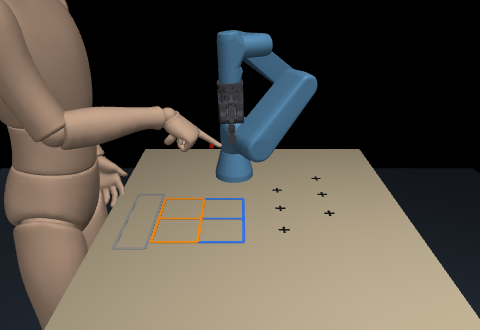
\includegraphics[height=2.95cm]{figures/point.png}\par\vspace{0.6em}
      {\large\textbf{Hướng dẫn}}\par\vspace{0.3em}
      {\small T1 · chỉ tay $\to$ robot lấy, đặt}
    \column{0.31\textwidth}\centering
      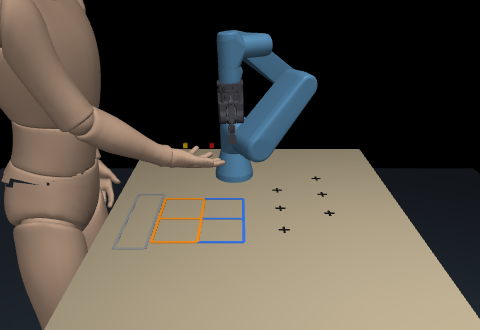
\includegraphics[height=2.95cm]{figures/palm.png}\par\vspace{0.6em}
      {\large\textbf{Cộng tác}}\par\vspace{0.3em}
      {\small T2 · trao vật cho người}\par
      {\small T3 · mang cốc cho người}
    \column{0.31\textwidth}\centering
      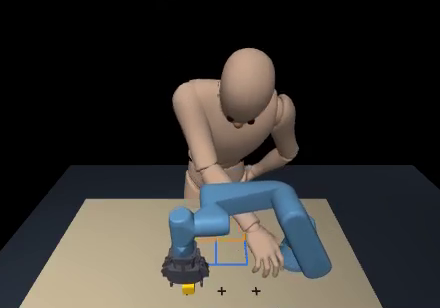
\includegraphics[height=2.95cm]{figures/intrude.png}\par\vspace{0.6em}
      {\large\textbf{Xâm nhập}}\par\vspace{0.3em}
      {\small T4 · robot nhường người}
  \end{columns}
  \vspace{1.6em}
  {\color{hot}\textbf{+ T5}}\ \ người đổi ý giữa chừng
\end{frame}

% =====================================================================
\begin{frame}{Thiết kế thí nghiệm $2\times2$}
  \centering
  \begin{tikzpicture}[font=\small,
      cell/.style={rounded corners=4pt, minimum width=3.6cm, minimum height=1.45cm, align=center}]
    \node[font=\normalsize] at (2,3.55) {Không có ý định};
    \node[font=\normalsize\bfseries, hot] at (6,3.55) {Có ý định};
    \node[anchor=east, align=right, font=\normalsize] at (-0.1,2.4) {Dữ liệu\\\textbf{chờ rõ}};
    \node[anchor=east, align=right, font=\normalsize] at (-0.1,0.6) {Dữ liệu\\\textbf{phản hồi sớm}};
    \node[cell, fill=line!60] at (2,2.4) {{\LARGE\bfseries A}\\[-1pt]\gray{cơ sở}};
    \node[cell, fill=line!60] at (6,2.4) {{\LARGE\bfseries C}};
    \node[cell, fill=line!60] (B) at (2,0.6) {{\LARGE\bfseries B}};
    \node[cell, fill=hot, text=white] (D) at (6,0.6) {{\LARGE\bfseries D}\\[-1pt]mô hình chính};
    \draw[{Stealth}-{Stealth}, hot, thick] (B.south) to[bend right=20]
      node[below, font=\small] {so sánh chính} (D.south);
  \end{tikzpicture}

  \vspace{0.5em}
  \gray{Cùng ACT · cùng episode · cùng cấu hình huấn luyện}\par
  \vspace{0.5em}
  Kỳ vọng: {\color{hot}\textbf{(D $-$ B) $>$ (C $-$ A)}}\quad
  \gray{\small intent có ích nhất khi phải phản hồi sớm}
\end{frame}

% =====================================================================
\begin{frame}{Đã làm được}
  \begin{columns}[t,onlytextwidth]
    \column{0.58\textwidth}
      \renewcommand{\arraystretch}{1.55}
      \begin{tabular}[t]{@{}cl@{}}
        \done & Môi trường: UR3e + người, 5 nhiệm vụ \\
        \done & Expert chờ rõ + dữ liệu: 559 episode \\
        \done & Đánh giá vòng kín, chỉ số HRI \\
        \half & Token ý định: đã chốt v3, chưa cài \\
        \todo & \gray{Expert sớm (theo quan sát) + dữ liệu} \\
      \end{tabular}
    \column{0.42\textwidth}
      \textbf{Huấn luyện}\par\vspace{0.8em}
      \begin{tikzpicture}[font=\small]
        \foreach \m/\y in {A/0, B/-0.8, C/-1.6, D/-2.4} {
          \node[anchor=east, font=\normalsize\bfseries] at (-0.15,\y) {\m};
          \fill[line!70, rounded corners=2pt] (0,\y-0.17) rectangle (2.6,\y+0.17);
        }
        \fill[accent, rounded corners=2pt] (0,-0.17) rectangle (1.95,0.17);
        \node[anchor=west] at (2.7,0) {15k / 20k};
        \node[anchor=west, mute] at (2.7,-0.8) {chờ dữ liệu};
        \node[anchor=west, mute] at (2.7,-1.6) {chưa train};
        \node[anchor=west, mute] at (2.7,-2.4) {chờ dữ liệu};
      \end{tikzpicture}
  \end{columns}
\end{frame}

% =====================================================================
\begin{frame}{Kết quả A (15k step): thành công}
  \begin{columns}[c]
    \column{0.68\textwidth}
      \begin{tikzpicture}
        \begin{axis}[
            ybar, bar width=11pt, width=\linewidth, height=5.4cm,
            ymin=0, ymax=112, ytick={0,50,100},
            symbolic x coords={T1,T2,T3,T4,T5}, xtick=data,
            xticklabels={T1\\[-2pt]{\scriptsize lấy--đặt}, T2\\[-2pt]{\scriptsize trao vật},
                         T3\\[-2pt]{\scriptsize mang cốc}, T4\\[-2pt]{\scriptsize nhường},
                         T5\\[-2pt]{\scriptsize đổi ý}},
            xticklabel style={align=center, font=\small},
            yticklabel style={font=\scriptsize, mute},
            ylabel={\small Thành công (\%)}, ylabel style={mute},
            axis lines*=left, axis line style={line}, major tick style={draw=none},
            enlarge x limits=0.14,
            legend style={draw=none, font=\small, at={(0.5,1.03)}, anchor=south,
                          legend columns=2, /tikz/every even column/.append style={column sep=10pt}},
            area legend]
          \addplot[fill=line, draw=none] coordinates {(T1,100) (T2,100) (T3,100) (T4,100) (T5,100)};
          \addplot[fill=accent, draw=none, nodes near coords,
                   every node near coord/.append style={font=\scriptsize, ink}]
            coordinates {(T1,96) (T2,81) (T3,85) (T4,8) (T5,33)};
          \legend{Expert, A}
        \end{axis}
      \end{tikzpicture}
    \column{0.28\textwidth}\centering
      {\fontsize{40}{44}\selectfont\bfseries\color{accent}63\%}\par
      \vspace{0.2em}
      A, toàn bộ tập eval\par
      \vspace{0.8em}
      \gray{Expert: 100\%}\par
      \gray{\small 263 episode, vòng kín}
  \end{columns}
\end{frame}

% =====================================================================
\begin{frame}{Kết quả A (15k step): tốc độ}
  \centering
  \vspace{0.6em}
  {\small
  \renewcommand{\arraystretch}{1.5}
  \begin{tabular}{@{}l c c c c c@{}}
    \toprule
    & T1 & T2 & T3 & T4 & T5 \\[-3pt]
    & \gray{\scriptsize lấy--đặt} & \gray{\scriptsize trao vật} & \gray{\scriptsize mang cốc}
    & \gray{\scriptsize nhường} & \gray{\scriptsize đổi ý} \\
    \midrule
    \textbf{CT} (s) $\downarrow$ \gray{\scriptsize hoàn thành} & 13,1 / 12,7 & 14,0 / 13,5 & 17,1 / 16,0 & -- & 19,0* / 22,4 \\
    \textbf{TSync} (s) $\downarrow$ \gray{\scriptsize lệch nhịp} & -- & 3,4 / 2,7 & 9,2 / 8,0 & -- & -- \\
    \textbf{Rsp} (s) $\downarrow$ \gray{\scriptsize trễ dừng} & -- & -- & -- & \textbf{0,54} / 0,19 & -- \\
    \bottomrule
  \end{tabular}}

  \vspace{1.2em}
  A chậm hơn expert \textbf{0,4--1,1 s} · dừng khi bị chen tay chậm \textbf{gần 3 lần}\par
  \vspace{0.8em}
  \gray{\scriptsize A / Expert · chỉ số kiểu HRIBench (công thức của đồ án) · CT chỉ tính episode thành công · *T5: 16/48 episode}
\end{frame}

% =====================================================================
\begin{frame}{Vấn đề đang gặp}
  \vspace{1em}
  \begin{itemize}\setlength{\itemsep}{1.1em}\large
    \item Expert sớm cũ \textbf{đọc đáp án mô phỏng} \gray{\small $\to$ sửa theo v3, kiểm tra lại seed}
    \item T4: robot \textbf{chưa nhường kịp} khi người chen tay
    \item T5: \textbf{đổi ý} còn thấp
    \item Rất nhạy với \textbf{cách chạy chuỗi hành động}
          \gray{\small(không ensembling: 0/55 episode)}
  \end{itemize}
\end{frame}

% =====================================================================
\begin{frame}{Kế hoạch 4 tuần}
  \centering
  \begin{tikzpicture}[font=\small, x=2.0cm, y=0.52cm]
    % cột tuần
    \foreach \w/\d [count=\i from 0] in {Tuần 1/{06--12/10}, Tuần 2/{13--19/10},
                                          Tuần 3/{20--26/10}, Tuần 4/{27/10--02/11}} {
      \node[align=center] at (\i+0.5,0.95) {\textbf{\w}\\[-1pt]{\scriptsize\color{mute}\d}};
      \draw[line] (\i,0.2) -- (\i,-9.3);
    }
    \draw[line] (4,0.2) -- (4,-9.3);
    % hàng công việc: nhãn / bắt đầu / kết thúc / màu
    \foreach \t/\a/\b/\c [count=\r from 1] in {
        Chốt cách chạy chunk/0/0.35/accent,
        Expert sớm theo quan sát/0.1/0.8/accent,
        {Thu dữ liệu sớm (± train lại A)}/0.75/1.4/accent,
        Token intent v3 trong ACT/0/1/hot,
        Model dự đoán intent/0.5/2/hot,
        {Train B, B+pose, C, D}/1.3/2.8/accent,
        {Eval + đổi / bỏ intent}/2.2/3.5/accent,
        Viết luận văn/2.6/4/mute} {
      \node[anchor=east] at (-0.08,-\r) {\t};
      \fill[\c, rounded corners=2pt] (\a+0.03,-\r-0.22) rectangle (\b-0.03,-\r+0.22);
    }
    % mốc
    \node[anchor=east, mute] at (-0.08,-9) {Mốc};
    \fill[ink] (2.8,-9) +(0,0.2) -- +(0.08,0) -- +(0,-0.2) -- +(-0.08,0) -- cycle;
    \node[anchor=east, font=\scriptsize] at (2.73,-9) {đủ A--D (1 seed)};
    \fill[ink] (4,-9) +(0,0.2) -- +(0.08,0) -- +(0,-0.2) -- +(-0.08,0) -- cycle;
    \node[anchor=east, font=\scriptsize] at (3.93,-9) {bản thảo};
  \end{tikzpicture}

  \gray{\scriptsize $\sim$12 lần train kể cả seed thêm ($\sim$10 giờ/lần): GTX 1650 + Colab T4}
\end{frame}

% =====================================================================
\begin{frame}[plain]
  \centering
  \vfill
  {\color{accent}\rule{1.5cm}{3pt}}\par\vspace{0.6cm}
  {\LARGE\bfseries Xin cảm ơn!}
  \vfill
\end{frame}

\end{document}
